\documentclass[11pt,a4paper]{article}
\usepackage[utf8]{inputenc}
\usepackage[spanish]{babel}
\usepackage{amsmath}
\usepackage{amsfonts}
\usepackage{amssymb}
\usepackage{graphicx}
\usepackage{hyperref}
\usepackage{pdflscape}
\usepackage{subcaption}
\usepackage{geometry}
\geometry{a4paper, margin=2.5cm}

\usepackage{fancyhdr}
\usepackage{tikz}
\usetikzlibrary{babel}

% Definición de estilo para páginas apaisadas con número rotado
\fancypagestyle{lscape}{
    \fancyhf{}
    \renewcommand{\headrulewidth}{0pt}
    \fancyfoot[C]{
        \begin{tikzpicture}[remember picture,overlay]
            \node[rotate=90, anchor=center, xshift=0cm, yshift=1cm] at (current page.east) {\thepage};
        \end{tikzpicture}
    }
}

\begin{document}
\renewcommand{\figurename}{Figura}

\begin{titlepage}
    \centering
    \vspace*{1cm}
    
    {\Huge \textbf{Informe de Proyecto: Detección y Mapeo Georreferenciado de Residuos mediante Enjambre UAV} \par}
    \vspace{2cm}
    
    \vspace{2cm}
    
    {\Large \textbf{Hugo Sevilla Martínez}} \par
    {\large \texttt{DNI: [48798351X]}} \par
    \vspace{0.5cm}
    {\Large \textbf{Hugo López Pastor}} \par
    {\large \texttt{DNI: [53979557Y]}} \par
    \vspace{1cm}
    
    {\large Grado en Ingeniería Robótica} \par
    
    \vfill
    
    
\includegraphics[width=0.4\textwidth]{img/ua_logo.png} \par
    
\end{titlepage}

\newpage
\tableofcontents
\newpage

\section{Objetivos}
El objetivo de este proyecto es diseñar, modelar y simular un enjambre de drones (UAVs) coordinados para detectar y mapear basura acumulada en las playas. Queremos crear un entorno de simulación realista usando ROS 2 y Gazebo Harmonic, integrando los modelos físicos de los drones, sus sensores, visión artificial con YOLOv8 y un algoritmo para calcular la posición real de cada residuo. Con esto, buscamos automatizar la búsqueda de basura y crear un mapa que sirva para facilitar las tareas de limpieza.

\section{Software Empleado}
El desarrollo de este sistema se ha llevado a cabo sobre una máquina con Linux nativo utilizando las siguientes herramientas:
\begin{itemize}
    \item \textbf{Ubuntu} 24.04 LTS.
    \item \textbf{ROS 2} Jazzy Jalisco.
    \item \textbf{Gazebo} Harmonic.
    \item \textbf{RViz2} como herramienta de visualización.
    \item \textbf{Python 3} para los nodos de control, visión y consolidación de mapas.
    \item \textbf{XACRO} como preprocesador de archivos URDF.
    \item \textbf{Ultralytics (YOLOv8)} y \textbf{OpenCV} para el procesamiento de inferencia visual.
    \item \textbf{Matplotlib} para la generación dinámica del mapa de residuos.
\end{itemize}

\section{Manual de Ejecución}
Para desplegar la simulación completa, que permite lanzar de manera paramétrica múltiples drones interactuando coordinadamente en el entorno, se deben seguir estos pasos utilizando tres terminales independientes:

\begin{enumerate}
    \item \textbf{Preparación del Entorno (Workspace)}: Situándose en la raíz del workspace con los paquetes clonados (\texttt{uav\_gazebo}, \texttt{uav\_description}, \texttt{uav\_control}, \texttt{uav\_vision}), se deberá compilar e iniciar el entorno:
    \begin{verbatim}
colcon build --symlink-install
source install/setup.bash
    \end{verbatim}

    \item \textbf{Terminal 1: Lanzar el Entorno Físico (Gazebo)}: Instancia el mundo con la textura de arena, los modelos 3D de residuos y el número deseado de robots (por defecto, $N=3$).
    \begin{verbatim}
ros2 launch uav_gazebo multi_uav.launch.py robots:=3
    \end{verbatim}

    \item \textbf{Terminal 2: Lanzar la Inferencia Visual y Mapeo}: Arranca los nodos de detección YOLO, los nodos de georreferenciación individual y el consolidador global de mapa. El parámetro \texttt{show\_gui:=false} suprime las ventanas de vídeo para optimizar el rendimiento de la CPU ya que hacen que la simulación vaya excesivamente lenta.
    \begin{verbatim}
ros2 launch uav_vision multi_vision.launch.py robots:=3 show_gui:=false
    \end{verbatim}

    \item \textbf{Terminal 3: Lanzar la Patrulla Sincronizada}: Inicia el algoritmo de barrido tipo \textit{lawnmower}. Los drones despegarán, se dirigirán a sus puntos de inicio, esperarán la confirmación por red de todos sus compañeros y comenzarán la exploración simultánea.
    \begin{verbatim}
ros2 launch uav_control multi_patrol.launch.py robots:=3
    \end{verbatim}
\end{enumerate}

El resultado final se actualizará cada 10 segundos en los archivos \texttt{mapa\_residuos.csv} y \texttt{mapa\_residuos.png} generados en la raíz del *workspace*.

\section{Desarrollo Técnico}
Para implementar el sistema de monitoreo, se ha diseñado una arquitectura distribuida y modular donde cada robot opera de forma independiente y coordina sus esfuerzos con los demás de manera asíncrona. La Figura~\ref{fig:nodo_architecture} detalla el flujo de información desde la simulación de sensores en Gazebo, pasando por el procesamiento individual en ROS 2, hasta la consolidación final en el mapa.

\begin{figure}[htbp]
    \centering
    \begin{tikzpicture}[
        node distance=1.5cm,
        node_block/.style={draw, rectangle, rounded corners, minimum width=2.8cm, minimum height=0.8cm, align=center, fill=blue!8, draw=blue!50, thick, font=\small},
        sensor_block/.style={draw, rectangle, rounded corners, minimum width=2.8cm, minimum height=0.8cm, align=center, fill=orange!8, draw=orange!50, thick, font=\small},
        global_block/.style={draw, rectangle, rounded corners, minimum width=3.2cm, minimum height=0.8cm, align=center, fill=green!5, draw=green!40!black!50, thick, font=\small},
        output_block/.style={draw, rectangle, minimum width=2.8cm, minimum height=0.8cm, align=center, fill=red!5, draw=red!50, thick, font=\small},
        arrow/.style={arrows={-stealth}, thick, draw=black!70},
        double_arrow/.style={arrows={stealth-stealth}, thick, draw=black!70},
        label_text/.style={font=\scriptsize\itshape, color=black!80}
    ]
        % Gazebo Simulator container
        \draw[dashed, fill=gray!5, draw=gray!40, thick] (-0.5, 0.5) rectangle (3.5, -6.8);
        \node at (1.5, 0.2) [font=\bfseries\small] {Gazebo (Simulación)};
        
        \node (camera) at (1.5, -0.5) [sensor_block] {Cámara RGB};
        \node (gps) at (1.5, -1.8) [sensor_block] {GPS (NavSat)};
        \node (altimeter) at (1.5, -3.1) [sensor_block] {Altímetro (Lidar)};
        \node (odom) at (1.5, -4.4) [sensor_block] {Odometría (Odom)};
        \node (cmd_vel) at (1.5, -5.8) [sensor_block] {cmd\_vel (Actuador)};

        % UAV Nodes Container
        \draw[dashed, fill=blue!2, draw=blue!30, thick] (4.8, 0.5) rectangle (8.8, -6.8);
        \node at (6.8, 0.2) [font=\bfseries\small] {Nodos UAV ($uav_i$)};
        
        \node (yolo) at (6.8, -0.8) [node_block] {yolo\_detector};
        \node (georef) at (6.8, -2.5) [node_block] {georeferencer};
        \node (patrol) at (6.8, -5.1) [node_block] {patrol.py};

        % Global system
        \node (sync) at (12.2, -5.1) [global_block] {Tópico de Sinc.\\ \texttt{/patrol\_sync}};
        \node (consolidator) at (12.2, -2.5) [global_block] {map\_consolidator};
        
        \node (csv) at (12.2, -0.5) [output_block] {\texttt{mapa\_residuos.csv}};
        \node (png) at (12.2, -1.4) [output_block] {\texttt{mapa\_residuos.png}};

        % Connections
        \draw [arrow] (camera) -- (yolo) node[midway, above, label_text] {/image\_raw};
        \draw [arrow] (yolo) -- (georef) node[midway, right, label_text] {/detections};
        
        \draw [arrow] (gps) -- (georef) node[midway, above, label_text] {/gps};
        \draw [arrow] (altimeter) -- (georef) node[midway, above, label_text] {/scan\_alt};
        
        \draw [arrow] (odom) -- (patrol) node[midway, above, label_text] {/odom};
        \draw [arrow] (patrol) -- (cmd_vel) node[midway, left, label_text] {/cmd\_vel};
        
        \draw [double_arrow] (patrol) -- (sync) node[midway, above, label_text] {Sinc. Estado};
        \draw [arrow] (georef) -- (consolidator) node[midway, above, label_text] {/detections\_georef};
        
        \draw [arrow] (consolidator) -- (csv);
        \draw [arrow] (consolidator) -- (png);

    \end{tikzpicture}
    \caption{Diagrama de arquitectura de nodos ROS 2 y flujo de datos de simulación/procesamiento.}
    \label{fig:nodo_architecture}
\end{figure}

\subsection{Configuración del Entorno Físico (Gazebo)}
Para la simulación, empezamos diseñando un entorno exterior en el archivo \texttt{outdoor.world}. Para que la simulación fuese visualmente realista y la red neuronal pudiese detectar los residuos correctamente, configuramos un terreno de arena clara de alta resolución y colocamos diferentes tipos de basura fotorrealista a lo largo de la playa.

Usamos tanto modelos nativos descargados de Gazebo Fuel (como cajas de cartón o latas de refresco) como modelos 3D externos importados de internet para tener más variedad de formas y texturas (Figura~\ref{fig:3d_models}). Tuvimos que ajustar a mano sus escalas, rotaciones y pesos en Gazebo para que se integraran bien en la arena y las físicas del simulador respondieran correctamente.

\begin{figure}[htbp]
    \centering
    \begin{subfigure}[b]{0.45\textwidth}
        \centering
        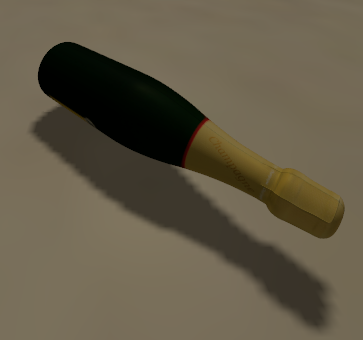
\includegraphics[width=\textwidth]{img/bottle.png}
        \caption{Modelo externo: Botella de plástico.}
        \label{fig:bottle_model}
    \end{subfigure}
    \hfill
    \begin{subfigure}[b]{0.45\textwidth}
        \centering
        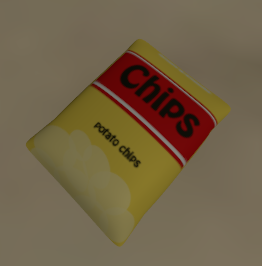
\includegraphics[width=\textwidth]{img/chips.png}
        \caption{Modelo externo: Bolsa de snacks.}
        \label{fig:chips_model}
    \end{subfigure}
    \caption{Ejemplo de modelos 3D externos de residuos integrados en la simulación.}
    \label{fig:3d_models}
\end{figure}

\begin{figure}[htbp]
    \centering
    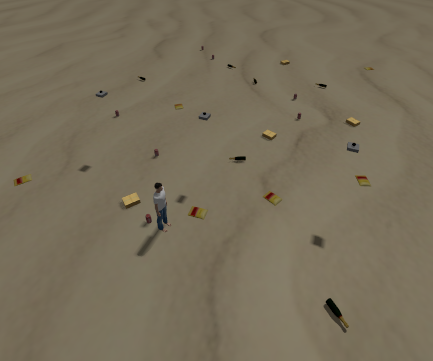
\includegraphics[width=0.8\textwidth]{img/entorno.png}
    \caption{Entorno de simulación en Gazebo (\texttt{outdoor.world}) con el enjambre desplegado sobre la zona de residuos modelados en 3D.}
    \label{fig:gazebo_world}
\end{figure}

\subsection{Optimización del Modelo URDF mediante XACRO}
Como ya hicimos en las prácticas de clase, el modelado del dron se ha hecho con un archivo \textbf{URDF} estructurado mediante \textbf{XACRO} (XML Macros). En lugar de escribir un único archivo gigante y difícil de entender, dividimos el modelo en varios archivos modularizados:

\begin{itemize}
    \item \textbf{Modelo Base (\texttt{uav.xacro})}: El archivo principal que une todo el chasis del dron (\textit{base\_link}), las hélices y llama al resto de ficheros.
    \item \textbf{Propiedades Comunes (\texttt{common\_}\allowbreak\texttt{properties.xacro})}: Guarda las constantes, colores, texturas y las fórmulas para calcular las inercias de forma automática.
    \item \textbf{Sensores}: Archivos como \texttt{camera.xacro}, \texttt{altimeter.}\allowbreak\texttt{xacro}, \texttt{gps.xacro}, \texttt{lidar.xacro} e \texttt{imu.xacro} con sus respectivos sensores y plugins.
    \item \textbf{Actuador de Vuelo (\texttt{flight\_}\allowbreak\texttt{control.xacro})}: Llama al plugin de Gazebo para mover los motores y que el dron responda físicamente al empuje.
    \item \textbf{Aislamiento por Prefijos}: Añadimos el argumento \texttt{prefix} para poder lanzar varios drones a la vez sin que choquen los nombres de los enlaces o tópicos en ROS 2 (por ejemplo, tener \texttt{uav1/base\_link} y \texttt{uav2/base\_link} por separado).
\end{itemize}

\begin{figure}[htbp]
    \centering
    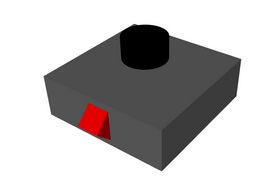
\includegraphics[width=0.6\textwidth]{img/modelo.png}
    \caption{Visualización limpia del modelo cinemático URDF del UAV base en RViz2.}
    \label{fig:rviz_drone}
\end{figure}

\subsection{Percepción: Integración de Sensores}
Cada dron lleva equipados cinco sensores en sus respectivos archivos \texttt{xacro}, que nos dan los datos necesarios para volar y detectar la basura:

\begin{itemize}
    \item \textbf{Cámara RGB (\texttt{camera.xacro})}: Apunta hacia el suelo con una resolución de $640 \times 480$ píxeles y un campo de visión (HFOV) de 1.089 radianes. Sirve para capturar el vídeo que procesará la red neuronal.
    \item \textbf{Altímetro (\texttt{altimeter.xacro})}: Un sensor Lidar de un solo rayo apuntando hacia abajo. Mide la distancia al suelo, lo que nos ayuda a mantener el dron a 2.5 metros de altura de crucero y a hacer el cálculo de la georreferenciación.
    \item \textbf{NavSat / GPS (\texttt{gps.xacro})}: Sensor GPS que nos da la latitud y longitud global del dron, imprescindible para colocar los residuos en el mapa.
    \item \textbf{Lidar 360º (\texttt{lidar.xacro})}: Sensor láser en la parte superior del chasis para escanear obstáculos en plano, pensado para esquivar objetos en el futuro.
    \item \textbf{IMU (\texttt{imu.xacro})}: Unidad de medición inercial para medir aceleraciones y velocidades de giro, lo que ayuda a mantener estable el chasis del dron en el aire.
\end{itemize}

\subsection{Arquitectura Multi-Robot y Control Distribuido}
La lógica de navegación y coordinación se gestiona de forma totalmente descentralizada mediante el nodo \texttt{patrol.py}. Para que los drones no choquen y cubran toda la zona rápido, dividimos el área de la playa en franjas horizontales paralelas, asignando una a cada dron.

\subsubsection{Subdivisión del Área y Generación de Trayectorias}
La playa está acotada en el eje Y por el intervalo $[Y_{\text{min}}, Y_{\text{max}}] = [-7.0, 7.0]$ metros. La anchura $w_y$ de la franja de cada dron se calcula de forma automática según los drones activos $N$:
\begin{equation}
w_y = \frac{Y_{\text{max}} - Y_{\text{min}}}{N}
\end{equation}

Para un dron con identificador $i \in \{1, 2, \dots, N\}$, su zona asignada en el eje Y es:
\begin{equation}
Y_i \in [Y_{\text{min}} + (i - 1)w_y, \; Y_{\text{min}} + i \cdot w_y]
\end{equation}

Dentro de su franja, cada dron realiza un barrido de ida y vuelta (tipo \textit{lawnmower}) en el eje X (de $2.0$ a $20.0$ metros), con un paso lateral de $\Delta y = 3.0$ metros. El punto de inicio de la exploración se calcula en el centro de su primera pasada para que la cobertura sea perfecta:
\begin{equation}
y_{\text{start}, i} = (Y_{\text{min}} + (i - 1)w_y) + \min\left(\frac{\Delta y}{2.0}, \frac{w_y}{2.0}\right)
\end{equation}

A partir de este punto, los waypoints se van incrementando sucesivamente en $\Delta y$ alternando el sentido en el eje X. Al estar las franjas físicamente separadas, garantizamos que los drones patrullan en paralelo de forma segura y sin peligro de chocar.

\subsubsection{Máquina de Estados y Protocolo de Sincronización}
Para coordinar a los drones sin necesitar una estación central que les envíe órdenes, programamos en el nodo de control una máquina de estados para cada dron con las siguientes fases:
\begin{itemize}
    \item \textbf{\texttt{TAKEOFF}}: El dron sube en vertical hasta llegar a la altura de crucero $z_{\text{target}} = 2.5$ metros.
    \item \textbf{\texttt{GOTO\_START}}: Vuela directo hacia el punto inicial de su franja de barrido ($W_0$).
    \item \textbf{\texttt{WAIT\_SYNC}}: Al llegar a $W_0$, se queda en vuelo estacionario (*hover*) y publica su estado en el tópico \texttt{/patrol\_sync}.
    \item \textbf{\texttt{PATROL}}: Cuando comprueba que los $N$ drones del enjambre están listos en el tópico, empieza a patrullar en paralelo siguiendo su trayectoria.
    \item \textbf{\texttt{FINISHED}}: Al terminar el barrido, el dron vuelve a su punto de despegue y aterriza apagando los motores.
\end{itemize}

\subsubsection{Clasificación y Flujo de Comunicación Multi-Robot}
Para analizar la coordinación del enjambre utilizando los conceptos vistos en clase, la interacción entre los drones se clasifica de la siguiente manera:

\begin{enumerate}
    \item \textbf{Comunicación Explícita (Directa):}
    Se produce cuando los drones se envían mensajes directos de datos por la red para coordinarse:
    \begin{itemize}
        \item \textbf{Sincronización de inicio (\texttt{/patrol\_}\allowbreak\texttt{sync}):} Durante la espera en vuelo estacionario (\texttt{WAIT\_}\allowbreak\texttt{SYNC}), cada dron publica su estado "listo" (mediante un mensaje \texttt{String}). Todos leen este tópico para hacer un quórum (comprobación de que están los $N$ drones listos) antes de empezar a patrullar a la vez. Este mecanismo actúa como un protocolo de confirmación o \textit{handshake} digital, muy similar al utilizado mediante señales físicas de I/O en la práctica 2.
        \item \textbf{Envío de detecciones (\texttt{/detections\_}\allowbreak\texttt{georeferenced}):} Cada dron transmite su lista de basura georreferenciada (\texttt{Detection2DArray}) directamente al nodo central \texttt{map\_}\allowbreak\texttt{consolidator.py} para actualizar el mapa.
    \end{itemize}
    
    \item \textbf{Comunicación Implícita (Indirecta o Estigmergia):}
    Se da cuando los robots obtienen información del entorno o de los compañeros sin necesidad de enviarse mensajes directos por la red:
    \begin{itemize}
        \item \textbf{Sensores Locales:} Los drones utilizan su propia cámara, GPS y altímetro para tomar medidas locales de forma individual y autónoma, permitiéndoles navegar sin sobrecargar el canal de comunicaciones ni depender de una red centralizada para el vuelo básico.
        \item \textbf{Estigmergia Pasiva:} En robótica de enjambres, la estigmergia representa la comunicación indirecta a través de la modificación del medio físico (como las feromonas de las hormigas). En nuestro proyecto, los drones cooperan de forma indirecta registrando sus hallazgos en un archivo común compartido (\texttt{mapa\_residuos.csv}). De este modo, los drones no necesitan comunicarse entre sí las posiciones de basura detectadas; simplemente modifican el "mapa del entorno común" y el consolidador unifica los datos.
    \end{itemize}

    \item \textbf{Paradigma de Coordinación (CTDE):}
    El enjambre sigue el paradigma de \textbf{Entrenamiento Centralizado con Ejecución Descentralizada} (\textit{Centralized Training with Decentralized Execution - CTDE}). En nuestro caso, la consolidación de los datos es centralizada (el nodo central recoge todo y crea el CSV global), pero el guiado y el vuelo de cada dron es completamente descentralizado y autónomo. Esto hace que el sistema sea muy robusto, ya que si un dron falla, los demás siguen volando y cubriendo sus zonas sin verse afectados.
\end{enumerate}

\begin{landscape}
\pagestyle{lscape}
\begin{figure}[p]
    \centering
    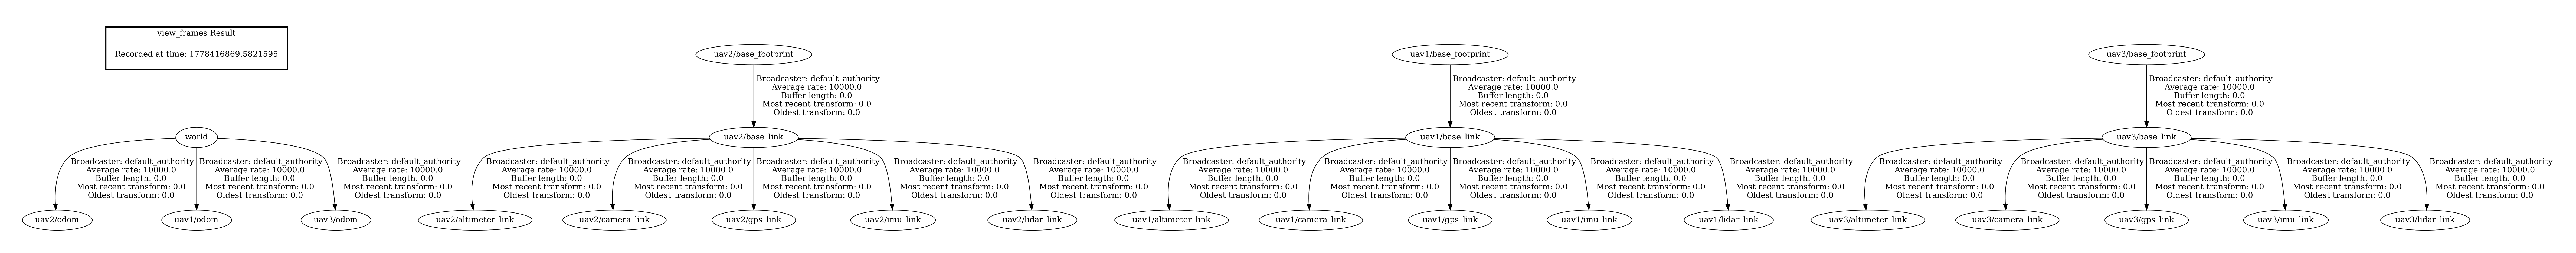
\includegraphics[width=\linewidth,height=0.8\textheight,keepaspectratio]{img/tf_tree_multi.png}
    \caption{Árbol de transformaciones (TF Tree) del sistema multi-robot. Todos los drones (uav1, uav2, uav3) cuelgan del frame maestro \texttt{world} y sus transformaciones están correctamente aisladas por namespaces.}
    \label{fig:gazebo_multi_tf}
\end{figure}
\end{landscape}
\pagestyle{plain}

\subsection{Visión Artificial y Posicionamiento GPS}
El procesamiento de imágenes y mapa se realiza en el paquete \texttt{uav\_vision}. Este paquete se encarga de procesar el vídeo de la cámara, detectar la basura, calcular su posición en coordenadas reales y guardarlo en el mapa final.

\subsubsection{Detección de Objetos en Tiempo Real (YOLOv8)}
En el nodo \texttt{yolo\_detector.py} nos suscribimos al tópico de la cámara del dron (\texttt{/uav\_i/}\allowbreak\texttt{camera/}\allowbreak\texttt{image\_raw}). Su funcionamiento es el siguiente:
\begin{enumerate}
    \item Recibe la imagen de la cámara de ROS y la convierte a una matriz OpenCV usando la librería \texttt{CvBridge} para poder procesar la imagen con código de Python.
    \item Le pasamos la imagen a la red neuronal YOLOv8 utilizando el modelo preentrenado \texttt{taco.pt} (entrenado con el dataset de basura \textit{TACO}), usando un umbral de confianza de $0.20$ para detectar objetos.
    \item Para cada trozo de basura detectado, calculamos el centro de su recuadro en píxeles $(u, v)$, lo metemos en un mensaje de tipo \texttt{Detection2DArray} y lo publicamos en el tópico \texttt{/uav\_i/yolo/detections}.
\end{enumerate}

\begin{figure}[htbp]
    \centering
    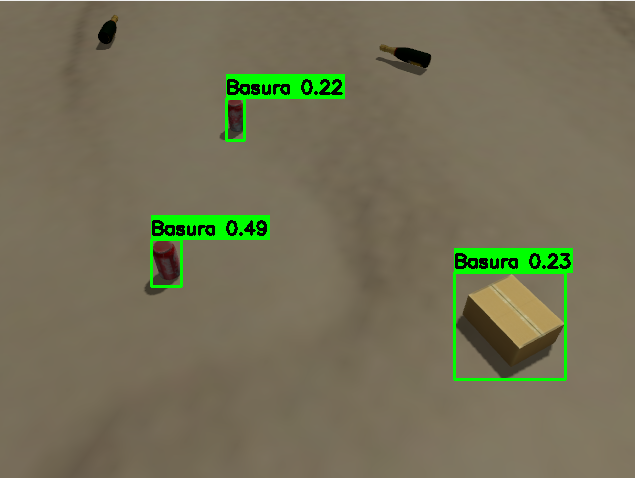
\includegraphics[width=0.7\textwidth]{img/inferencia_yolo.png}
    \caption{Inferencia en tiempo real del flujo de vídeo usando YOLOv8 sobre objetos de la simulación.}
    \label{fig:yolo_detection}
\end{figure}

\subsubsection{Motor Matemático de Georreferenciación}
El nodo \texttt{georeferencer\_node.py} se encarga de calcular la posición real en coordenadas GPS (latitud y longitud) a partir de los píxeles $(u, v)$ de la imagen. La lógica matemática sigue estos tres pasos:

\begin{enumerate}
    \item \textbf{Cálculo de la Distancia Focal en Píxeles ($f_{\text{px}}$):}
    Usando la anchura de la imagen ($640$ píxeles) y el campo de visión horizontal de la cámara ($\text{HFOV} = 1.089$ radianes), calculamos la distancia focal virtual en píxeles:
    \begin{equation}
    f_{\text{px}} = \frac{640}{2 \cdot \tan\left(\frac{\text{HFOV}}{2}\right)}
    \end{equation}

    \item \textbf{Proyección a Coordenadas Métricas del Dron ($d_x, d_y$):}
    Calculamos el desvío en píxeles de la detección respecto al centro de la imagen ($u_c, v_c = 320, 240$):
    \begin{align}
    \Delta u &= u - 320 \\
    \Delta v &= v - 240
    \end{align}
    Y usando la altura ($h$) medida por el altímetro, estimamos la distancia en metros de la basura respecto al dron:
    \begin{align}
    d_y &= \frac{\Delta u \cdot h}{f_{\text{px}}} \\
    d_x &= \frac{\Delta v \cdot h}{f_{\text{px}}}
    \end{align}
    donde $d_x$ es la distancia hacia adelante/atrás y $d_y$ es la distancia lateral hacia los lados en el eje del dron.

    \item \textbf{Conversión Geodésica a Grados (WGS84 local):}
    Con la posición GPS actual del dron ($\text{lat}_{\text{drone}}, \text{lon}_{\text{drone}}$) y sabiendo que un grado terrestre equivale a unos $111\,132$ metros ($R_{\text{deg}}$), sumamos el desplazamiento en metros para obtener la posición GPS exacta de la basura:
    \begin{align}
    \text{lat}_{\text{target}} &= \text{lat}_{\text{drone}} + \frac{d_x}{R_{\text{deg}}} \\
    \text{lon}_{\text{target}} &= \text{lon}_{\text{drone}} + \frac{d_y}{R_{\text{deg}} \cdot \cos\left(\frac{\pi \cdot \text{lat}_{\text{drone}}}{180}\right)}
    \\
    \text{alt}_{\text{target}} &= h
    \end{align}
    Esta posición calculada se publica en el tópico \texttt{detections\_georeferenced} dentro del namespace de cada dron.
\end{enumerate}

\subsubsection{Consolidación Global y Filtrado de Duplicados}
El nodo central \texttt{map\_}\allowbreak\texttt{consolidator.py} escucha las posiciones GPS de todos los drones a la vez. Cuando le llega una nueva detección $P_{\text{new}} = (\text{lat}_{\text{new}}, \text{lon}_{\text{new}})$, para no guardar la misma basura varias veces (si la ven varios drones o el mismo dron en fotos seguidas), calculamos la distancia en metros a las basuras ya registradas usando la \textbf{Fórmula del Haversine}:
\begin{align}
\Delta \phi &= \frac{\pi}{180} (\text{lat}_{\text{new}} - \text{lat}_j) \\
\Delta \lambda &= \frac{\pi}{180} (\text{lon}_{\text{new}} - \text{lon}_j) \\
a &= \sin^2\left(\frac{\Delta \phi}{2}\right) + \cos\left(\frac{\pi \cdot \text{lat}_{\text{new}}}{180}\right)\cos\left(\frac{\pi \cdot \text{lat}_j}{180}\right)\sin^2\left(\frac{\Delta \lambda}{2}\right) \\
c &= 2 \cdot \operatorname{atan2}\left(\sqrt{a}, \sqrt{1-a}\right) \\
d &= R_{\text{Earth}} \cdot c
\end{align}
donde $R_{\text{Earth}} = 6\,371\,000$ metros es el radio medio de la Tierra.

Si la distancia calculada es menor de $2.0$ metros ($d_{\text{min}}$), consideramos que es el mismo objeto y lo descartamos. Si es mayor, lo guardamos en memoria, lo escribimos con su marca de tiempo en el archivo \texttt{mapa\_residuos.csv} y redibujamos el mapa dinámico en \texttt{mapa\_residuos.png} (Figura~\ref{fig:map_final}) de forma asíncrona mediante Matplotlib.

\begin{figure}[htbp]
    \centering
    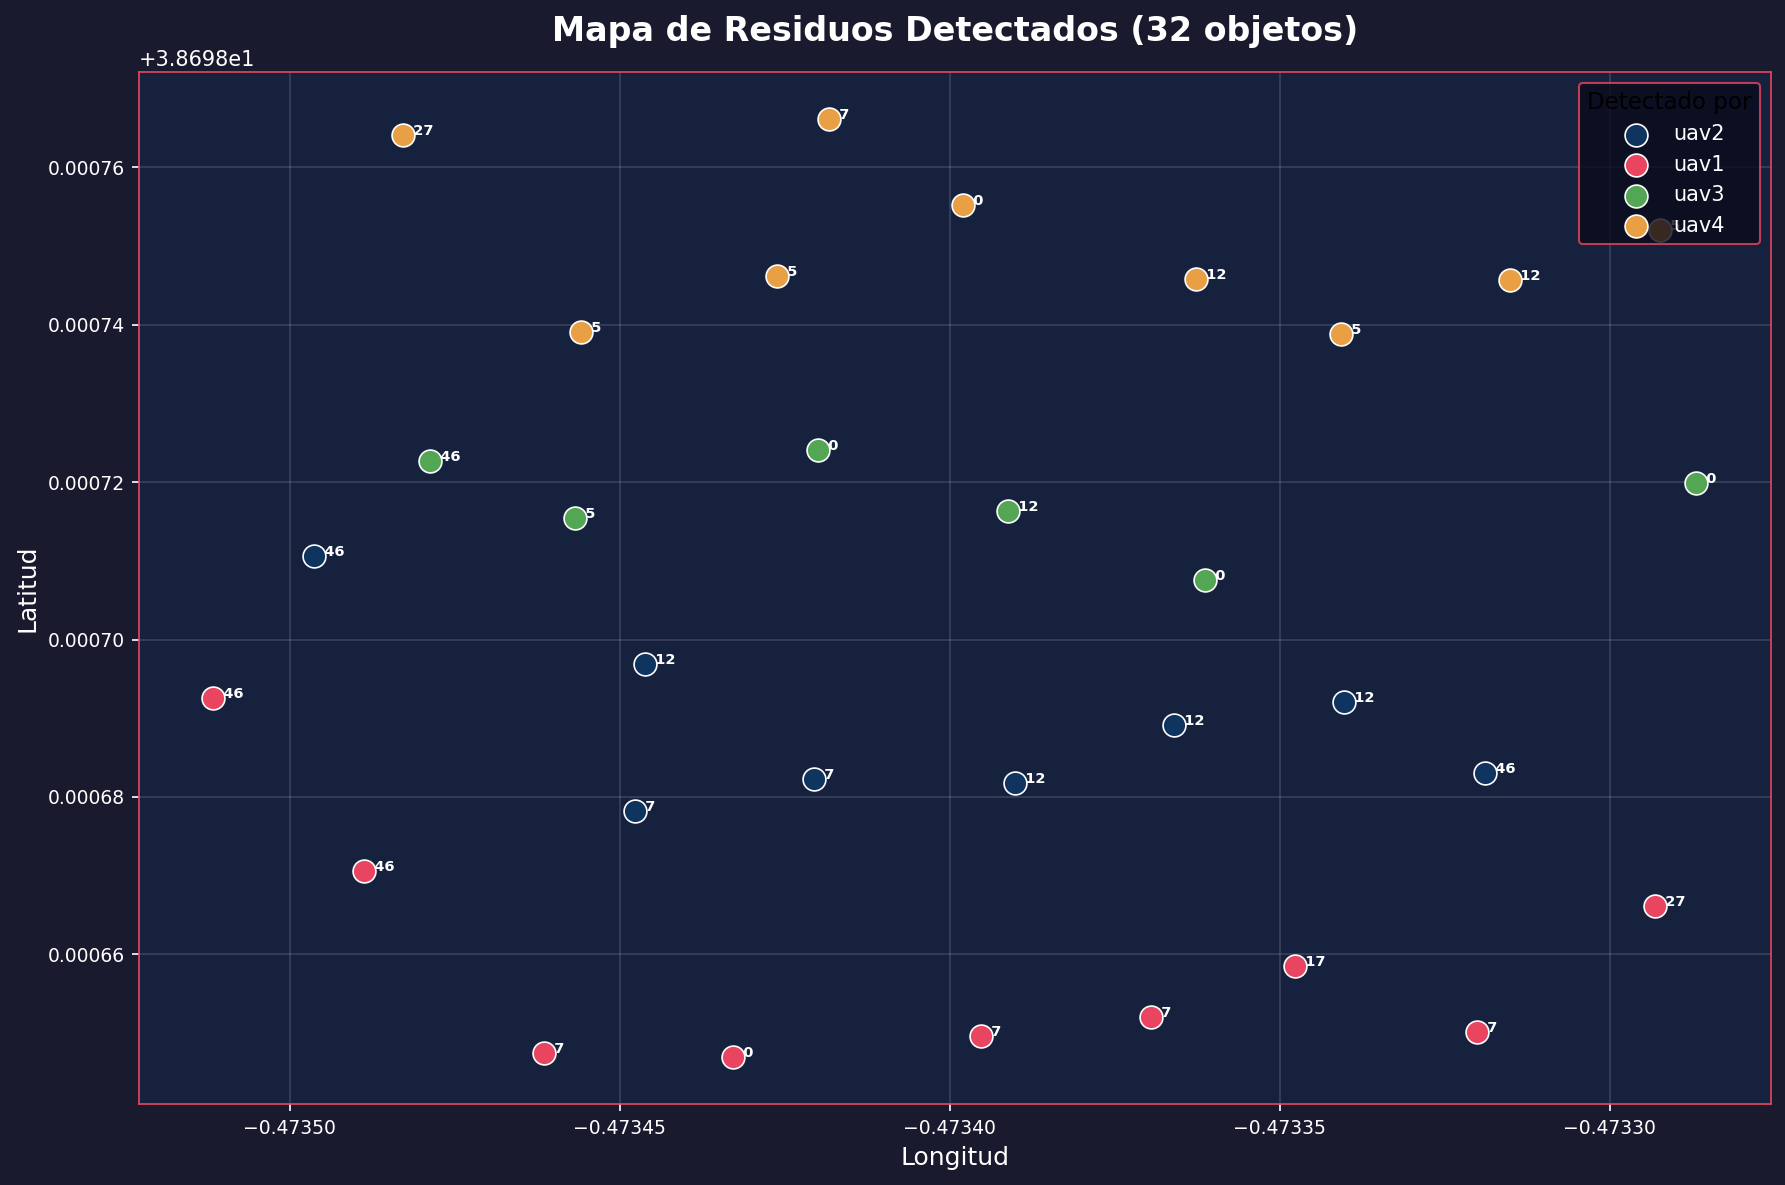
\includegraphics[width=0.8\textwidth]{img/mapa_residuos.png}
    \caption{Mapa generado automáticamente en Matplotlib indicando la tipología de residuo y el dron detector.}
    \label{fig:map_final}
\end{figure}

\section{Estructura del Sistema de Ficheros}
El proyecto está organizado en varios paquetes de ROS 2 para que el código quede más ordenado y sea más fácil de gestionar:

\begin{description}
    \item[\texttt{uav\_gazebo/}] Contiene el mundo de simulación y los archivos launch para lanzar todo en Gazebo.
    \begin{itemize}
        \item \texttt{worlds/outdoor.world}: Define el entorno de la playa, la iluminación y coloca los modelos 3D de la basura.
        \item \texttt{launch/multi\_uav.launch.py}: Lanza los drones en Gazebo aplicando los namespaces correspondientes para que no haya conflictos.
    \end{itemize}

    \item[\texttt{uav\_description/}] Contiene los archivos para definir cómo es el dron físicamente y cómo se visualiza.
    \begin{itemize}
        \item \texttt{urdf/*}: Archivos XACRO que definen el chasis, los motores y los sensores del dron.
        \item \texttt{rviz/uav.rviz}: Configuración de RViz2 para ver el modelo del dron de forma limpia.
    \end{itemize}

    \item[\texttt{uav\_control/}] Controla el vuelo y comportamiento del enjambre de drones.
    \begin{itemize}
        \item \texttt{uav\_control/patrol.py}: Nodo que lleva la máquina de estados, el guiado de los drones y el barrido coordinado de la playa.
    \end{itemize}

    \item[\texttt{uav\_vision/}] Se encarga del procesamiento de imágenes y la creación del mapa de residuos.
    \begin{itemize}
        \item \texttt{yolo\_detector.py}: Nodo que coge las imágenes de la cámara, las pasa por YOLOv8 y publica las detecciones.
        \item \texttt{georeferencer\_node.py}: Nodo que calcula la posición GPS real de la basura a partir de los píxeles de la imagen.
        \item \texttt{map\_consolidator.py}: Nodo central que elimina los duplicados con la fórmula del Haversine y guarda el mapa final en CSV e imagen PNG.
    \end{itemize}
\end{description}

\section{Dificultades y Resoluciones}
Durante el desarrollo del proyecto surgieron varios problemas y dificultades que tuvimos que ir resolviendo:

\begin{enumerate}
    \item \textbf{Detección de objetos 3D con YOLOv8 (Sim2Real)}: Al principio, el modelo de YOLOv8 (entrenado con fotos reales) no detectaba bien los objetos 3D de Gazebo porque eran muy lisos y no tenían texturas reales. Para solucionarlo, ajustamos el umbral de confianza (\textit{confidence threshold}) a $0.20$ para hacerlo más sensible y cambiamos la textura del suelo del simulador por una arena clara que contrastara más con la basura. De esta forma, la red neuronal pudo empezar a detectar los objetos por sus formas básicas sin confundirse con el suelo.

    \item \textbf{Despegue y avance descompasado del enjambre}: Como cada dron tarda un tiempo ligeramente diferente en despegar e ir a su posición inicial, los primeros que llegaban empezaban a patrullar antes de que los demás estuvieran listos, desorganizando el barrido. Lo solucionamos creando un tópico común llamado \texttt{/patrol\_sync} donde los drones publican su estado. Ninguno empieza a patrullar hasta comprobar en este tópico que todos los drones del enjambre están listos en sus puntos de salida.

    \item \textbf{Ralentización del ordenador por las ventanas de vídeo (GUI)}: Ejecutar tres nodos de visión a la vez (uno por dron) mostrando la imagen de la cámara en tiempo real con las cajas y textos de OpenCV consumía demasiados recursos, haciendo que el ordenador fuera lentísimo y se congelara la simulación. La solución fue añadir el parámetro \texttt{show\_gui:=false} para ejecutar el procesamiento de visión de fondo sin abrir ventanas gráficas. Así, el procesamiento interno sigue funcionando exactamente igual pero el simulador va mucho más rápido y fluido.
\end{enumerate}

\section{Conclusiones y Trabajo Futuro}
Como conclusión general, el proyecto demuestra que un enjambre de drones es muy útil para buscar y mapear residuos en una playa de forma automatizada. Al usar ROS 2 y Gazebo, hemos comprobado que si aumentamos el número de drones ($N$), el tiempo necesario para explorar toda la zona disminuye de forma proporcional. Además, al no haber un nodo o controlador central que maneje el vuelo, el sistema es mucho más seguro y robusto: si un dron tiene un problema y se cae, los demás pueden seguir patrullando sus zonas asignadas sin enterarse.

Como trabajos futuros o posibles mejoras para ampliar el proyecto, se proponen las siguientes ideas:
\begin{itemize}
    \item \textbf{Procesamiento a bordo (Edge Computing)}: En un escenario real, transmitir vídeo en alta definición por Wi-Fi o radio desde cada dron a un ordenador central consume mucho ancho de banda y da retrasos. Una mejora importante sería meter en cada dron una tarjeta pequeña de procesamiento (como una NVIDIA Jetson Nano o una Google Coral). Así, el algoritmo YOLOv8 correría directamente en el propio dron y solo tendríamos que enviar por red las coordenadas GPS del residuo detectado, que es un mensaje muy ligero.
    \item \textbf{Simulación con PX4 (SITL/HITL)}: Sustituir el plugin de movimiento de Gazebo por una conexión con el simulador de controladora de vuelo de PX4. Esto permitiría simular el vuelo usando el mismo software que llevaría un dron real, lo que haría la simulación mucho más fiel a la realidad.
    \item \textbf{Reentrenamiento del modelo (Fine-tuning)}: Sacar fotos de los objetos 3D directamente dentro del propio simulador de Gazebo para reentrenar el modelo de YOLOv8 con ellas. Esto ayudaría a que la red neuronal reconozca los modelos virtuales sin ningún fallo antes de hacer pruebas de vuelo reales.
    \item \textbf{Recogida activa de basura}: Ir un paso más allá del simple mapeo y diseñar un sistema para recoger la basura. Se podría añadir un brazo o una pinza pequeña a los drones para que la recojan ellos mismos, o bien añadir robots terrestres al enjambre que reciban las coordenadas GPS enviadas por los drones y vayan por tierra a recoger los residuos.
\end{itemize}

\section{Uso de Herramientas de IA}
Durante el desarrollo del proyecto hemos utilizado Inteligencia Artificial como ChatGPT o Gemini para ayudarnos a depurar el código Python, configurar el XACRO de los drones en Gazebo Harmonic, y corregir la redacción y formato de esta memoria.

\begin{thebibliography}{9}
\bibitem{ros2_docs}
Open Robotics.
\textit{Documentación Oficial de ROS 2 Jazzy Jalisco}.
\url{https://docs.ros.org/en/jazzy/}

\bibitem{gazebo_docs}
Open Source Robotics Foundation.
\textit{Gazebo Harmonic Documentation}.
\url{https://gazebosim.org/docs/harmonic}

\bibitem{taco_dataset}
TACO - Trash Annotations in Context.
\textit{Repositorio de imágenes e identificadores de residuos}.
\url{http://tacodataset.org/}

\bibitem{ultralytics_yolo}
Ultralytics.
\textit{YOLOv8 Architecture and Object Detection}.
\url{https://docs.ultralytics.com/}

\bibitem{haversine_formula}
Wikipedia.
\textit{Fórmula del Haversine - Cálculo de distancias geodésicas}.
\url{https://es.wikipedia.org/wiki/F%C3%B3rmula_del_haversine}
\end{thebibliography}

\end{document}
